\documentclass[conference]{IEEEtran}
\usepackage[utf8]{inputenc}
\usepackage{ifpdf}
\renewcommand{\sfdefault}{cmss}
\renewcommand{\rmdefault}{cmr}
\renewcommand{\ttdefault}{cmtt}
\usepackage[english,russian]{babel}
\usepackage[pdftex]{graphicx}
\usepackage{caption}
\usepackage[colorlinks,filecolor=blue,citecolor=green,unicode,pdftex]{hyperref}
\usepackage{cmap}
\usepackage{amsmath,amssymb}
\usepackage[mathcal]{euscript}
\hypersetup{colorlinks=true, linkcolor=blue, citecolor=blue, filecolor=blue, urlcolor=blue, pdftitle=1, pdfauthor=, pdfsubject=, pdfkeywords=}
\usepackage[noadjust]{cite}
\renewcommand{\citedash}{--}

\sloppy
\clubpenalty=0
\widowpenalty=0
\raggedbottom

\begin{document}

\title{Язык программирования роботов в терминах потоков данных}

\author{
	\IEEEauthorblockN{Г.А. Зимин}
	\IEEEauthorblockA{
		Санкт-Петербургский государственный университет\\
		Кафедра системного программирования\\
		Email: zimin.grigory@gmail.com
	}
	
	\and

	\IEEEauthorblockN{Д.А. Мордвинов}
	\IEEEauthorblockA{
		Санкт-Петербургский государственный университет\\
		Кафедра системного программирования\\
		Email: mordvinov.dmitry@gmail.com
	}
}

\maketitle

%``пульт'' поправить все ковычки

\begin{abstract}
В статье описывается язык программирования роботов в терминах потоков данных на основе модельно-ориентированного подхода. Дается краткий обзор языков программирования роботов. Рассматриваются подходы к реализации систем управления роботами. В заключение представлено решение типовой задачи создания системы управления на описанном языке с применением архитектуры Брукса. 
\end{abstract}

\section{Введение}
Взаимодействие с роботами и языки программирования для них --- это актуальная тема исследований: статьи, освещающие связанные с ними вопросы, постоянно обозреваются на крупных конференциях, к примеру, ICRA\footnote{http://www.icra2016.org/ [Дата обращения: 10 марта 2016]}, IROS\footnote{http://www.iros2016.org/ [Дата обращения: 10 марта 2016]}. Последние три десятилетия продолжается активное изучение и исследование возможностей применения  визуальных языков программирования --- каждый год проводятся крупные конференции, такие как VL/HCC\footnote{https://sites.google.com/site/vlhcc2016/ [Дата обращения: 10 марта 2016]}. В робототехнике визуальные языки программирования также нашли свое применение~\cite{banyasad2000visual,simpson2006mobile,simpson2008visual,posso2011process,diprose2011ruru}. Они позволяют быстрее создавать и нагляднее отображать системы управления роботами, обучать робототехнике школьников --- примерами этого могут служить различные среды программирования роботов для начинающих, такие как NXT-G\footnote{http://www.legoengineering.com/program/nxt-g/ [Дата обращения: 10 марта 2016]}, TRIK Studio\footnote{http://www.trikset.com/ [Дата обращения: 10 марта 2016]}, ROBOLAB\footnote{http://www.legoengineering.com/program/robolab/ [Дата обращения: 10 марта 2016]}. 

Программы управления роботом по своей природе реактивны: они обрабатывают данные, непрерывно приходящие с множества датчиков, и посылают команды на приводы. В силу этого для программирования роботов хорошо подходят реактивные языки, или языки программирования потоков данных (data flow languages). Эти языки также активно развивались от текстовых к широко распространенным сейчас визуальным языкам потоков данных~\cite{johnston2004advances}. В случае программирования потоков данных наглядность визуальных языков особо превосходит текстовые, так как сами потоки данных явно отображены на диаграмме. Существуют большие и сложные среды программирования, такие как LabVIEW\footnote{http://www.ni.com/labview/ [Дата обращения: 10 марта 2016]} и Simulink\footnote{http://www.mathworks.com/products/simulink/ [Дата обращения: 10 марта 2016]}, которые предоставляют большой и даже громоздкий набор библиотек для программирования роботов. Подробнее про языки программирования роботов будет сказано в разделе~\ref{sec:Overview}.

Для обучения основам робототехники и кибернетики существует большое количество конструкторов роботов, таких как линейка конструкторов LEGO MINDSTORMS\footnote{http://www.lego.com/en-us/mindstorms/products [Дата обращения: 10 марта 2016]}, конструктор TRIK\footnote{http://blog.trikset.com/p/blog-page\_6355.html/ [Дата обращения: 10 марта 2016]}.
Подавляющее большинство современных языков программирования, используемых для обучения программированию на них, основаны на модели потока управления, а не потока данных. При этом во время их освоения зачастую появляется ощущение неудобства решения на них типовых задач управления роботом. Дополнительная <<ступень>> в виде простого в освоении потокового языка была бы весьма полезной при переходе от учебных языков программирования к тем, что используются в индустрии. Целью данной работы является создание такого языка программирования конструкторов роботов TRIK.


Остаток работы устроен следующим образом: в разделе~\ref{sec:Overview} дан краткий обзор существующих визуальных языков программирования для роботов и их применения, в разделе~\ref{sec:Brooks} обозреваются архитектуры, на которых может быть построена система управлениями роботами, в разделах~\ref{sec:lang},~\ref{sec:example} дается описание языка и его применение к решению задачи управления роботом при помощи оператора с автоматическим избеганием столкновений, наконец, в разделе~\ref{sec:conclusion} коротко будут сформулированы итоги работы. 

\section{Обзор современных языков программирования роботов}
\label{sec:Overview}
Среды программирования роботов можно разделить на три класса: учебные, позволяющие программировать небольших роботов; промышленные, обладающие богатым инструментарием для создания систем управления роботов и различных моделей; академические, которые реализуют какие-либо интересные идеи, однако часто они либо недоступны для конечных пользователей, либо их стабильность оставляет желать лучшего. 

К учебным, к примеру, можно отнести среду разработки EV3 Software~\cite{3_rollins} для конструктора Lego Mindstorms EV3, среду разработки NXT-G\footnote{http://www.legoengineering.com/program/nxt-g/ [Дата обращения: 10 марта 2016]} и конструктор LEGO MINDSTORMS NXT и ROBOLAB\footnote{http://www.legoengineering.com/program/robolab/ [Дата обращения: 10 марта 2016]}, конструктор TRIK и среду программирования TRIK Studio\footnote{http://www.trikset.com/ [Дата обращения: 10 марта 2016]}. Упомянутые среды программирования позволяют с легкостью решать типовые задачи управления роботом: найти выход из лабиринта, проехать по линии, используя сенсоры, создавая примитивные системы управления для обучения пользователя основам программирования и управления роботами. Но своей простотой они обязаны слабой гибкости языка, по сути они предоставляют последовательную модель потока управления роботом, описанную наглядными графическими моделями.

В инженерной индустрии весьма популярна среда общего назначения LabVIEW компании National Instruments и визуальный потоковый язык программирования G, а также среда для моделирования динамических моделей и различных систем управления Simulink. Данные программные продукты предоставляют пользователю огромный набор моделей и библиотек для создания любых систем управления, испытательных стендов, систем реального времени, используя модельно-ориентированный подход. В частности, на LabVIEW возможно программирование небольших роботов. Хотя известны применения LabVIEW в образовательных целях~\cite{1_gomez-de-gabriel_mandow_fernandez-lozano_garcia-cerezo_2011}, большинство времени в образовательном процессе уходит на изучение самой среды, а не алгоритмов и подходов робототехники. Следует отметить, что эти среды распространяются под коммерческой лицензией.
%нужна статья про обучению школьников лабвью

Другой пример промышленной системы --- Microsoft Robotics Developer Studio (MSRDS)~\cite{jackson2007microsoft}, бесплатная для академического использования, удобная для программирования распределенных робототехнических систем в терминах потоков данных, компоненты которых представляются веб-сервисами. MSRDS официально поддерживает множество робототехнических платформ, среди которых есть LEGO NXT~\cite{kim2007programming}, для которого, однако отсутствует поддержка автономного режима. MSRDS обладает возможностью интеграции пользовательских робототехнических платформ, однако сама среда не поддерживается с 2014 года.
 
В данной области ведется множество исследовательских работ, к примеру, в диссертации~\cite{banyasad2000visual} описан визуальный язык программирования в терминах расширенных машин Мура,~\cite{simpson2008visual, posso2011process} описывают визуальный язык в терминах потоков данных с привязкой к языку программирования $occam\mbox{-}\pi$ и инструментарию $Transterpreter$, а также применение к управлению <<роем>> роботов. Работа~\cite{diprose2011ruru} описывает визуальный потоковый язык и среду для обучения новичков программированию роботов, среда предоставляет удобный интерфейс, однако полученная технология обладает недостаточными функциональными возможностями и требует значительной доработки, а также недоступна для конечных пользователей.

Исходя из результатов обзора ясно, что для создания и дальнейшей поддержки языка программирования в терминах потоков данных конструкторов роботов TRIK не подходит ни одна из упомянутых сред (в том виде, в котором она представлена на данный момент). При этом самым близким к желаемому является TRIK Studio, так как это единственная среда в открытом доступе с легко масштабируемой архитектурой, обладающей возможностью расширения новым визуальным языком программирования роботов и переиспользования кодовой базы таких <<рутинных>> операций, как взаимодействие с роботом.


\section{Архитектура Брукса}
\label{sec:Brooks}
С выходом статьи Родни Брукса~\cite{1_brooks_1986}, описывающей возможность проводить декомпозицию задачи управления роботом горизонтально на уровни ответственности, стало возможно проще и эффективнее решать <<составные>> задачи управления, как, например, задачи телеоператорского контроля балансирующего робота с автоматическим избеганием столкновений с препятствиями. Языки потоков данных удачно подходят для этой модели, что подтверждают неоднократные публикации на эту тему:~\cite{simpson2006mobile, banyasad2000visual,posso2011process,proetzsch2007behaviour}. В этой модели система управления представлена как набор уровней ответственности, которые отвечают за различные модели поведения робота и строятся последовательно. При этом, по очевидным причинам, упрощается масштабируемость системы и увеличивается ее отказоустойчивость.

	У архитектуры Брукса есть множество альтернатив, к примеру, <<Колония>> Джонотана Коннеля, архитектура <<выбора-действия>> Патти Мэйса, <<схема двигателя>> Рональда Аркина~\cite{simpson2009toward}, модель управления для системы Телеробота~\cite{albus1989nasa}. Однако среди упомянутых подходов подход Брукса является наиболее популярным, поэтому основополагающей концепцией разрабатываемого языка было решено сделать поддержку именно его.


\section{Описание языка}
\label{sec:lang}
Развитие модельно-ориентированного (\textit{DSM}) подхода~\cite{koznov2008} позволило быстро создавать достаточно сложные визуальные языки программирования. Среда программирования TRIK Studio является примером системы, созданной с применением DSM-подхода на базе платформы QReal~\cite{qrealMeta,kuzenkova2013qreal}. Основываясь на промышленном опыте разработчиков TRIK Studio, было решено создавать потоковый язык программирования роботов на базе платформы QReal. Первый прототип языка был создан в течение недели. На момент написания статьи язык и средства его поддержки находятся в активной разработке. Опишем некоторые особенности разрабатываемой технологии:

\begin{itemize}
\item Архитектура Брукса легко выражается средствами языка.
\item Диаграммы поведения роботов, так же как и в TRIK Studio, имеют возможность быть проинтерпретированными на двумерной имитационной модели робота. 
\item В ближайших планах стоит генерация диаграмм потоков данных в текстовые языки, используемые для программирования TRIK --- в первую очередь, JavaScript, F\#~\cite{kirsanov2014robotics} и Kotlin.
\end{itemize}

Элементами языка являются связи и блоки, опишем их конкретнее:

\begin{itemize}
\item \textit{Элемент потока данных}. Связь, реализующая поток для передачи данных. 
\item \textit{Блоки управления приводами}. Блоки, принимающие числовые значения, отвечающие за подачу импульсов на приводы (силовые моторы, сервомоторы и т.д.).
\item \textit{Блоки считывания данных с сенсоров}. Блоки, генерирующие соответствующие значения, которые подлежат дальнейшей обработке.
\item \textit{Блоки синхронизации и фильтрации}. Позволяют временно блокировать передачу данных, устанавливать количество наборов пропускаемых данных и время между отправками. 
\item \textit{Блоки поддержки устройств ввода}. Считывают данные с устройств операторского контроля (в данный момент поддержан только джойстик, в планах --- компьютерная мышь и клавиатура). 
\item \textit{Блоки рисования на экране}. Отвечают за векторное и растровое рисование на экране.
\item \textit{Блоки видеозрения}. Предоставляют доступ ко всем возможностям видеозрения контроллера TRIK.
\item \textit{Блоки взаимодействия между роботами}. Отвечают за групповую координацию роботов.
\item \textit{Блок текстового программирования}. Блок, позволяющий произвести обработку входных данных на текстовом языке (статически типизируемом диалекте Lua, поддержка которого <<унаследована>> от кодовой базы TRIK Studio). Чаще всего такой блок будет использоваться для задания математических операций над данными.
\item \textit{Блоки управляющих конструкций}. Включают циклы, условные развилки, множественный выбор, распараллеливание, подавление и ингибицию, блок <<Подпрограмма>> для переиспользования кода. Последние четыре блока обеспечивают поддержку архитектуры Брукса в языке.

\end{itemize} 

\section{Пример решения задачи}
\label{sec:example}
Рассмотрим задачу управления движением робота при помощи джойстика, при условии, что робот сам избегает лобовых столкновений с препятствиями. Предполагается, что программа пишется для двухколесного мобильного робота, оборудованного спереди инфракрасными датчиками расстояния, для управления колесами используются силовые моторы.

Разобьем задачу на два уровня поведения. Первый будет отвечать за обслуживание запросов пользователя. Второй будет ответственен за избегание столкновений: если робот близок к столкновению, то он должен уклониться от препятствия вне зависимости от того, что нажимает пользователь на пульте. 

Рассмотрим первый уровень (рис.~\ref{image:layer1}). Пользователь управляет роботом посредством джойстика. Джойстик генерирует данные, соответствующие нажатиям кнопок или манипулирований рычагом направления. Для простоты считаем, что нажатие любой кнопки завершит программу управления роботом. Данные с рычага преобразуются блоком текстового программирования в соответствующие импульсы моторов робота, которые в данном случае передаются <<заглушкам>>, которые связаны с выходными портами блока <<Подпрограмма>>. 
\begin{figure}[ht]
	\centering
	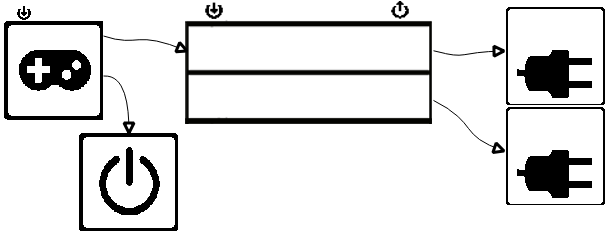
\includegraphics[width=3.5in]{pultLayer.png}
	\caption{Уровень управления с пульта.}
	\label{image:layer1}
\end{figure}

Рассмотрим второй уровень (рис.~\ref{image:layer2}): данные с датчиков расстояния собираются в вектор и передаются фильтру, который при опасности столкновения отправляет данные дальше в блок математической обработки (если условие не выполнилось, управление может быть передано по потоку <<ошибки>>, в данной программе этот поток не указан; также между проверками условия приходящие данные не обрабатываются (теряются) в течение установленного пользователем времени). В блоке математической обработки вычисляется мощность, которую необходимо подать на два мотора. Вычисленные значения передаются выходным портам.
\begin{figure}[ht]
	\centering
	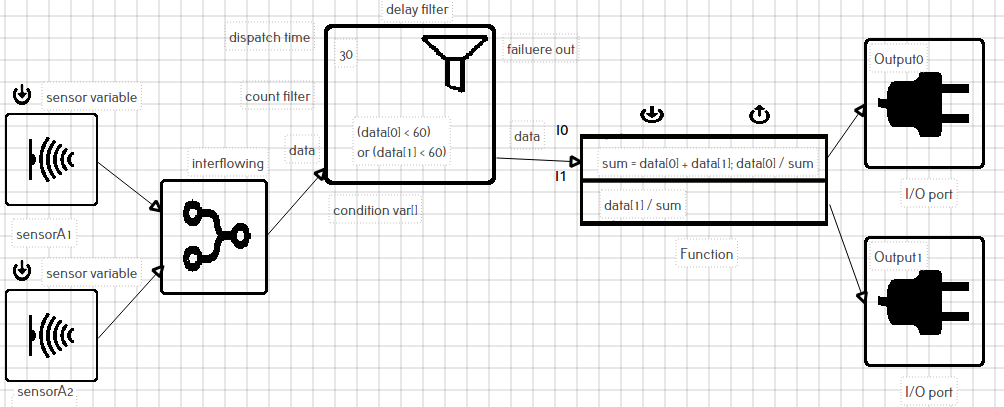
\includegraphics[width=3.5in]{collisionLayer.png}
	\caption{Уровень избегания столкновений.}
	\label{image:layer2}
\end{figure}

\begin{figure}[ht]
	\centering
	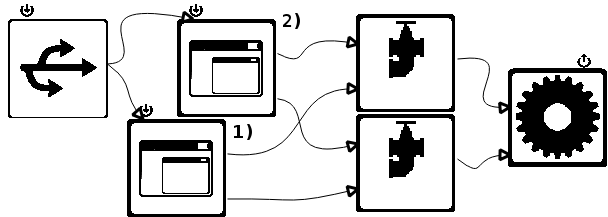
\includegraphics[width=3.5in]{programScreen.png}
	\caption{Программа управления роботом. 1 --- первый уровень, 2 ---второй .}
	\label{image:prog}
\end{figure}

На основе двух уровней поведения создаем управление роботом в модели Брукса (рис.~\ref{image:prog}). С помощью блока распараллеливания запускаем уровни поведения. Каждый уровень генерирует данные, соответствующие мощностям моторов, передаваемые на блок управления силовыми моторами. Так как второй уровень ответственности должен не позволить столкнуться с препятствием, его значения подавляют значения, полученные с первого уровня, с помощью блоков <<Подавления>>.


\section{Заключение}
\label{sec:conclusion}
На момент написания статьи был реализован прототип технологии программирования роботов TRIK в терминах потоков данных. Система предоставляет возможность интерпретации диаграмм на двумерной имитационной модели робота и (в ближайшем будущем) генерации кода из диаграмм в текстовые языки, используемые для программирования TRIK (JavaScript, F\# и Kotlin). Также технология предоставляет поддержку архитектуры Брукса на уровне языка, что продемонстрировано в статье на примере операторского управления роботом с автоматическим избеганием столкновений.

Полученная система может рассматриваться как платформа для дальнейших научных исследований. К примеру, интересной представляется автоматическая генерации метамодели языка по спецификациям промежуточного ПО (middleware) на роботе (к примеру, ROS\footnote{http://www.ros.org/ [Дата обращения: 10 марта 2016]}). Другим направлением возможной работы является описание строгой семантики языка для применения различных формальных методов анализа программ, выраженных в нем.

\newpage
\bibliographystyle{utf8gost705u}
\bibliography{bibliography}
\end{document}